%%%%%%%%%%%%%%%%%%%%%%%%%%%%%%%%%%%%%%%%%%%%%%%%%%%%%%%%%%%%%%%%%%%%%%%%%%%%%%%%%%%%%%%
%%%%%%%%%%%%%%%%%%%%%%%%%%%%%%%%%%%%%%%%%%%%%%%%%%%%%%%%%%%%%%%%%%%%%%%%%%%%%%%%%%%%%%%
% 
% This top part of the document is called the 'preamble'.  Modify it with caution!
%
% The real document starts below where it says 'The main document starts here'.


\documentclass[12pt]{article}

\usepackage{amssymb,amsmath,amsthm}
\usepackage[top=1in, bottom=1in, left=1.25in, right=1.25in]{geometry}
\usepackage{fancyhdr}
\usepackage{listings}
\usepackage{enumerate}
\usepackage{hieroglf}
\usepackage{oands}
\usepackage{arevmath}
\usepackage{relsize}
\usepackage{times,txfonts}
\usepackage{graphicx}
\usepackage{float}

\newtheoremstyle{homework}% name of the style to be used
  {18pt}% measure of space to leave above the theorem. E.g.: 3pt
  {12pt}% measure of space to leave below the theorem. E.g.: 3pt
  {}% name of font to use in the body of the theorem
  {}% measure of space to indent
  {\bfseries}% name of head font
  {:}% punctuation between head and body
  {2ex}% space after theorem head; " " = normal interword space
  {}% Manually specify head
\theoremstyle{homework} 

% Set up an Exercise environment and a Solution label.
\newtheorem*{exercisecore}{Exercise \@currentlabel}
\newenvironment{exercise}[1]
{\def\@currentlabel{#1}\exercisecore}
{\endexercisecore}

\newcommand{\localhead}[1]{\par\smallskip\noindent\textbf{#1}\nobreak\\}%
\newcommand\solution{\localhead{Solution:}}

%%%%%%%%%%%%%%%%%%%%%%%%%%%%%%%%%%%%%%%%%%%%%%%%%%%%%%%%%%%%%%%%%%%%%%%%
%
% Stuff for getting the name/document date/title across the header
\makeatletter
\RequirePackage{fancyhdr}
\pagestyle{fancy}
\fancyfoot[C]{\ifnum \value{page} > 1\relax\thepage\fi}
\fancyhead[L]{\ifx\@doclabel\@empty\else\@doclabel\fi}
\fancyhead[C]{\ifx\@docdate\@empty\else\@docdate\fi}
\fancyhead[R]{\ifx\@docauthor\@empty\else\@docauthor\fi}
\headheight 15pt

\def\doclabel#1{\gdef\@doclabel{#1}}
\doclabel{Use {\tt\textbackslash doclabel\{MY LABEL\}}.}
\def\docdate#1{\gdef\@docdate{#1}}
\docdate{Use {\tt\textbackslash docdate\{MY DATE\}}.}
\def\docauthor#1{\gdef\@docauthor{#1}}
\docauthor{Use {\tt\textbackslash docauthor\{MY NAME\}}.}
\makeatother

% Shortcuts for blackboard bold number sets (reals, integers, etc.)
\newcommand{\Reals}{\ensuremath{\mathbb R}}
\newcommand{\Nats}{\ensuremath{\mathbb N}}
\newcommand{\Ints}{\ensuremath{\mathbb Z}}
\newcommand{\Rats}{\ensuremath{\mathbb Q}}
\newcommand{\Cplx}{\ensuremath{\mathbb C}}
%% Some equivalents that some people may prefer.
\let\RR\Reals
\let\NN\Nats
\let\II\Ints
\let\CC\Cplx

%%%%%%%%%%%%%%%%%%%%%%%%%%%%%%%%%%%%%%%%%%%%%%%%%%%%%%%%%%%%%%%%%%%%%%%%%%%%%%%%%%%%%%%
%%%%%%%%%%%%%%%%%%%%%%%%%%%%%%%%%%%%%%%%%%%%%%%%%%%%%%%%%%%%%%%%%%%%%%%%%%%%%%%%%%%%%%%
% 
% The main document start here.

% The following commands set up the material that appears in the header.
\doclabel{Math 316: HW 3}
\docauthor{Stefano Fochesatto}
\docdate{\today}

\begin{document}


\textbf{Section 3.4}
\begin{enumerate}
\setcounter{enumi}{1}
\item  The following solution to the continued mean proportionals problem is often attributed to Plato, although
it could hardly be his in view of his objection to mechanical constructions. Consider two right triangles $ABC$ and 
$BCD$, lying on the same side of he common leg $BC$. Suppose that the hypotenuses $AC$ and $BD$ intersect perpendicularly
at point $P$, and are constructed in such a way that $AP= a$ and $DP = 2a$. Prove that $x = BP$ and $y = CP$ are the required mean proportionals between 
$a$ and $2a$, that is, 
\begin{equation*}
  \frac{a}{x} = \frac{x}{y} = \frac{y}{2a}.
\end{equation*}
\begin{center}
  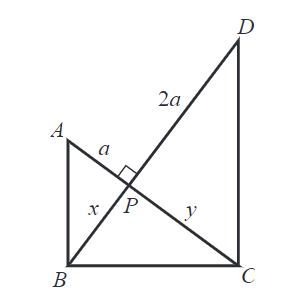
\includegraphics[width = .33\textwidth]{meanprop.png}
\end{center}
\textbf{Answer:} Note that since $ABC$ and $BCD$ are right triangles with the following property, 
\begin{equation*}
  \angle ABC = \angle DCB = 90^{\circ}
\end{equation*}  
Note that these angles sum to $180^{\circ}$ and are the interior angles to segments $AB$ and $DC$. Therefore by Euclid's Parallel postulate 
$AB$||$DC$. With segments $AC$ and $BD$ as transversals we get the following equalities through alternate interior angles.
\begin{equation*}
  \angle BAC = \angle DCA,
\end{equation*}
\begin{equation*}
  \angle ABD = \angle CDB.
\end{equation*}
Therefore we get $\triangle APB \sim \triangle CPD$ by AA similarity. Note that by the construction of point $P$ and vertical angles we know that,
\begin{equation*}
  \angle DPA = \angle BPC = \angle APB = \angle CPD = 90^{\circ}.
\end{equation*}  
Since the angles of  $\triangle BCD$ and $\triangle CPD$ sum $180^{\circ}$
we get the following through algebra, 
\begin{align*}
  \angle CDB + \angle DCP + 90^{\circ} &= \angle CDB + \angle CBD + 90^{\circ},\\
  \angle DCP &= \angle CBD.
\end{align*}
Note that $\angle CBP = \angle CBD = \angle DCP$ and $\angle BPC =\angle CPD$ therefore by AA similarity $\triangle BPC \sim \triangle CPD$. Thus by 
the transitivity of similar triangles we know that $\triangle APB \sim \triangle CPD \sim \triangle BPC$ and the desired proportional relationship,
\begin{equation*}
  \frac{a}{x} = \frac{x}{y} = \frac{y}{2a}
\end{equation*}
is derived from the ratio between the legs of each right triangle. 






\vspace{.5in}



\setcounter{enumi}{3}
\item
\textbf{Answer:} 
\vspace{.5in}



\end{enumerate}
\vspace{.5in}

\textbf{Intro to GeogGebra worksheet}



\textbf{Section 4.2}
\begin{enumerate}
\item 
\textbf{Answer:}
\vspace{.5in}

\setcounter{enumi}{6}
\item
\textbf{Answer:} 
\vspace{.5in}


\setcounter{enumi}{10}
\item
\textbf{Answer:} 
\vspace{.5in}





\setcounter{enumi}{11}
\item
\textbf{Answer:} 
\vspace{.5in}

\end{enumerate}
\vspace{.5in}



\textbf{Reflection:}
\begin{enumerate}
\item 
\item 
\end{enumerate}





\end{document}